\documentclass[12pt, titlepage]{article}

\usepackage{booktabs}
\usepackage{tabularx}
\usepackage{hyperref}
\usepackage{float}

\usepackage{graphicx}
\graphicspath{ {./coverage/} }

\hypersetup{
    colorlinks,
    citecolor=black,
    filecolor=black,
    linkcolor=red,
    urlcolor=blue
}
\usepackage[round]{natbib}

\title{SE 3XA3: Test Report\\Chrome Dino Runner}

\author{Team 1\#, Team Rex
		\\ Anjola Adewale and adewaa1
		\\ Chelsea Maramot and maramotc
		\\ Sheridan Fong and fongs7
}

\date{\today}


\begin{document}

\maketitle

\pagenumbering{roman}
\tableofcontents
\listoftables
\listoffigures


\newpage

\pagenumbering{arabic}
\newpage
\begin{table}[h]
\caption{\bf Revision History}
\begin{tabularx}{\textwidth}{p{3cm}p{2cm}X}
    \toprule {\bf Date} & {\bf Version} & {\bf Notes}\\
    \midrule
    February 4, 2022 & 0 & All team members\\
    \midrule
    April 10, 2022 & 1.0 & Sheridan Fong (updated functional tests)\\
    \midrule
    April 10, 2022 & 1.1 & Anjola Adewale (updated non-functional tests)\\
    \midrule
    April 11, 2022 & 1.2 & Chelsea Maramot (updated matrix and code coverage)\\
    \bottomrule
    
\end{tabularx}
\end{table}
\newpage

\section{Functional Requirements Evaluation}

Description of Tests: These tests ensure that the user is able to use the software according to the Software Requirement Specification (SRS). The following tests include the checking the functionalities of the Instructions, Leaderboard, Game Settings, and Game Track.

\subsection{E1: Viewing the Instructions Page}
The Instructions Page is fully functional. The user is able to access it by pressing the ``How to play" button in the Menu Page. The keyboard bindings are displayed in a comprehensive manner. The system then displays the Instructions page satisfying FR1. Finally, the user is able to transition back to the Menu Page from the Instructions Page satisfying FR2.

\subsection{E2: Viewing the Leaderboard}
The Leaderboard Page is fully functional. The user is able to access the Leaderboard Page from the Main Page by clicking the text. The system displays the top five scores of all users. This is different than FR3 as FR3 displays the top scores of the specific user. The leaderboard implemented does not filter the high scores by user and therefore FR5 is not met. The user can navigate back to the menu by pressing 'b' and therefore this satisfies FR4. 


\subsection{E3: Change Game Settings}
The Game Settings Page meets the functional requirements stated in the SRS. The user is able to transition from the Game Settings Page to the Menu Page and vice versa, as stated in FR6. Moreover, the game audio can be manipulated by the user within the Game Settings Page, as stated in FR7. Finally, FR8 states that themes must be displayed and the user is able to select a theme. This functional requirement has been met.

\subsection{E4: Playing the Game}
The game functions as proposed, the game displays the correct theme based off user input, the initial score is 0 and sound is outputted based on settings, this satisfies FR9, FR10, and FR11 respectively. The system starts gameplay when the user inputs any key not just WASD keys therefore FR12 fails. The game is controlled by WASD keys and arrow keys therefore satisfying FR13. The game awards points when the user moves and display's the current score to the screen, therefore FR14 and FR15 are satisfied. FR17 is satisfied as the system allows the user to replay the game and they can stop the game by pressing 'p' and return to the main menu. The user can only enter their username on the Main Page therefore FR18 fails. After game play the score is entered into the database. 


\section{Nonfunctional Requirements Evaluation}
\subsection{Look and Feel}	
LF1: The user interface consists of essential components relevant to the game such as the obstacles, and characters
LF2,LF3: Although we implemented two new themes, we left the original version of the game as a theme option. Therefore the game maintains the 90's arcade appearance.
LF4: The game is fully implemented in black and whit, therefore the  game colours do not distract the user's game play

\subsection{Usability}
UH1: The game was implemented to be controlled using two methods. The arrow keys and ``WASD" keys
UH2: Through survey testing we verified that the game has a simple main menu page which leads to the different game settings	UH3. Through survey testing we verified that the game was partially intuitive. Some users found that they had to perform "jumping" and ``ducking" actions earlier than anticipated in order to do die in the game.
UH4: The game instructions and settings are implemented in English
UH5: The theme of the game is easily adjustable. All a user has to do is navigate to the game page and select the theme they want.
UH6: User's that participated in the test group did not undergo any prior training before playing the game, thus this requirement is achieved
UH7: The instructions in the main menu are easy to understand as verified by survey testing
UH8:The game is delivered as an executable file, therefore there is a level of abstraction from the user
U9,UH10: These requirement were fully implemented, the game used common controls like the space-bar, arrow keys and ``WASD" keys to control the character.
UH11,UH12: Since the game a was fully implemented in black and white with large fonts, all accessibility requirements are satisfied
\subsection{Performance}
PE1: The scores are uploaded to the leaderboard in less than 10 seconds after game play. This was verified by using the time library in our code. 
PE2: The interface has a response time of less than 2 seconds. This was verified manually and through using the time library.   
PE3: The game updates the new status parameters such as game theme and audio settings within 5 seconds. This was verified manually. 
PE4: This functional requirement was not specific. Integer whole numbers for the game score were updated within 900 ms of changing. This was verified manually. 
PE5: The leaderboard is updated according to the top integer score, this was verified using manual and unit testing. 
PE6: The maximum latency is less then 900 ms when navigating between pages. This was verified by looking at the flags and when they changed using the time library. 
PE7: The game is only available to a single player at a time on a local device. However, multiple people can play the game on different local devices. Since, this requirement was not clearly defined it is partially satisfied. 
PE8: The game has a maximum of five users stored in the leaderboard. This was satisfied with manual and unit testing.
PE9: Developers are able to implement new features without compromising the functionality of the game. This was tested manually by the developers when implementing new features. The modular designed allowed for a relatively easy development process. 
PE10: The game maintains functionality with existing software until Spring 2022 (which is now), so this NFR is satisfied. 
PE11: The game plays with full functionality without internet connection, therefore this is satisfied. 
PE12: The game does not play on any operating system. This was proven through our usability tests when deploying it to other operating systems. 
PE13: This requirement is satisfied as the game is deployed using an executable file. 
PE14: This FR is not satisfied as additional instructions to download the executable is required. 
PE15: The game was released on April 5th 2022 and was ahead of the schedule release data by one week. Therefore, this requirement is satisfied. 

\subsection{Maintainability and Support}
MA1: This requirement is partially satisfied as it was not specific. All source code was updated with the latest changes before or on the day of scheduled dates. 
MA2: All source code is documented using Doxygen. This requirement is satisfied. 
MA3: The full project source code is available to Git users but you must first log-in to your Gitlab account to raise issues. Therefore, this requirement is partially satisfied. 
MA4: The game only runs on Windows therefore this requirement is partially satisfied. 

\subsection{Security Requirements}	
SR1: In the current implementation of the game, once the game is launched the user is not able to edit the Leaderboard. 
SR2: Users are permitted to change game settings through the user interface therefore the requirement is satisfied. 
SR3: The product does not protect itself from unauthorized user modifications, this is due to the download method for users. 
SR4: The user is able to modify the scores due to the download method. 
SR5: This is satisfied as the user can view other usernames and their corresponding high scores. 
SR6: This functional requirement is partially satisfied as our game has not been rigorously tested against unauthorized or undesirable software programs. There has been no issues thus far with harmful software. 

\subsection{Cultural and Political Requirements}
CP1: The game themes are not offensive to any cultures or religions therefore this requirement is satisfied. 
CP2: The game does not allow users to input offensive English user names. This was completed by having a dictionary of inappropriate usernames that the system checked for. The dictionary is currently only in English and therefore does not satisfy the requirement fully. 


\section{Automated Testing}
\subsubsection{Settings Page Tests}
	
\begin{enumerate}

\item{FS-SPT-1\\}

Initial State: audio variable = True
					
Input: Keyboard Input N or A 
					
Output: The audio variable will change based on the keyboard input. 


\item{FS-SPT-2\\}


Initial State: theme = `default'
					
Input: Keyboard Input ``1", ``2", or ``3"
					
Output: Based on the keyboard input, the theme variable value should change:``1" for the default dino theme, ``2" for the student theme and ``3" for the corona virus theme.
				
\end{enumerate}



\subsubsection{Leaderboard Tests}

\begin{enumerate}

\item{FST-LT-1\\}

Initial State: User is at the Restart screen waiting for an area to be selected(mouse event)
					
Input: User clicks on the area of the ``Leaderboard" text
					
Output: The Leaderboard page is displayed and contains up to five users and their scores.
					

\item{FST-LT-2\\}
					
Initial State: None, this function is called on a unit basis. However the score.txt file must be populated
					
Input: Leaders\_text (Python list containing top users and their score)
					
Output: Unit test passes if the users in the leader board (leaders\_text) have the highest recorded scores
					

% This should probably be on a restart page test
\item{FST-LT-4\\}
					
Initial State: Restart flag is set to True and game point is higher than the current user's highest score.
					
Input: Game points
					
Output: If game points is higher than the current user high score, unit test passes if the user's high score is updated to the game points.
					

\end{enumerate}

% \subsubsection{Gametrack Tests}

% \begin{enumerate}

% \end{enumerate}



\subsubsection{Instructions Page Tests}

\begin{enumerate}

\item{FST-IPT-1\\}
					
Initial State: Current page displayed within interface is the main menu page and instructions = False.
					
Input: User selects the area within the ``How to play" text
					
Output: The current page displayed on the interface will be the instructions page and instructions = True.
					
\item{FST-IPT-2\\}
					
Initial State: The Current page displayed within the interface is the instructions page.
					
Input: The user enters the associated keyboard exit key (``e").
					
Output: Current page displayed within the interface will transition to the main menu page.
					

\item{FST-IPT-3\\}
					
Initial State:  The game is paused and instructions = False.
					
Input: The user enters the associated keyboard (``i") input.
					
Output: Current page displayed within the interface will transition to the instructions page and instructions = True.



\end{enumerate}

% \subsubsection{Operating System Compatibility Test}

% \begin{enumerate}

% \item{FST-IPT-3\\}

% Type: Structural, Manual, Dynamic
					
% Initial State: Game is stored in an executable file and uploaded to Google drive
					
% Input: Download and launch the game on computers running on  Windows 10, macOS Sierra 10.12 and Linux Ubuntu 16.04.
					
% Output: Game should run successfully on any of these operating systems.
					
% How test will be performed: The executable file containing our program will be uploaded to Google drive.
% The test team will then download and execute the programs on systems running on Windows 10, macOS Sierra 10.12 and Linux Ubuntu 16.04. The test team will verify the successful run of the game on these systems
% \end{enumerate}



% \subsection{Tests for Nonfunctional Requirements}

% \subsubsection{Look and Feel}

% \paragraph{Style Requirements}

% \begin{enumerate}


% \item{NFS-1\\}

% Type: Functional, Manual, Dynamic 
					
% Initial State: The game executable file is loaded and is currently on the main page.
					
% Input/Condition: The test group are asked to inspect the interface and its design.
					
% Output/Result: Atleast 80\% of the test group will report that the game colours are not distracting and the 90's arcade appearance is maintained.
					

% \end{enumerate}


% \subsubsection{Usability}
		
% \paragraph{Ease of Use}

% \begin{enumerate}


% \item{NFS-2\\}

% Type: Functional, Manual, Dynamic 
					
% Initial State: Game is newly launched from an executable file and set up on a computer (Main Menu Page)
					
% Input/Condition: Users are asked to play the game
					
% Output/Result: Majority of the users are able to successfully play the game without any assistance from the development team
					

% \item{NFS-3\\}

% Type: Structural, Manual, Dynamic 
					
% Initial State: Game is stored in an executable file and uploaded to Google drive
					
% Input/Condition: The test group is asked to download and launch the game on their computers running Windows 10, macOS Sierra 10.12 or Linux Ubuntu 16.04.
					
% Output/Result: Users from the test group are successfully able to launch the game on their computers without assistance from the development team.


% \end{enumerate}

% \subsubsection{Precision Test}
% \begin{enumerate}
% \item{NFS-4\\}

% Type: Functional, Dynamic, Manual
					
% Initial State: The game is launched and user-input (keyboard or mouse) is expected
					
% Input: Using a stop watch, time how long it takes for the game to response (change page) after an input is entered.
					
% Output: The average response time should be less than two seconds

% % \end{enumerate}

% \subsubsection{Security Requirements}

% \paragraph{Access Requirements}
% \begin{enumerate}
% \item{NFS-5\\}

% Type: Functional, Dynamic, Manual
					
% Initial State: The interface is currently displaying the leaderboard page
					
% Input: User mouse and keyboard input

% Output: The user is not able to change the leaderboard names and high score.
					
% \end{enumerate}


% \subsubsection{Cultural and Political Requirements}

% \paragraph{Cultural Requirements}
% \begin{enumerate}
% \item{NFS-6\\}

% Type: Functional, Dynamic, Automated 
					
% Initial State: The game prompts the user for a username
					
% Input: Illegal username (e.g a swear word)
					
% Output: An error message should be displayed to inform the user of an illegal username

% % \end{enumerate}

% \section{Tests for Proof of Concept}

% Proof of Concept verifies and validates the method by which automated testing is performed. The testing for proof of concept will test the functionality of the game and game flow logic. 


% \subsection{Game Play}
		
% \paragraph{Game Track}

% \begin{enumerate}

% \item{POC-1\\}
					
% Initial State: Game track page is display to the screen and game points = 0
					
% Input: N/A
					
% Output: Game track is shown to the screen and updated score is in the top right corner. 
					
% \item{POC-2\\}

% Type: Functional, Dynamic, Manual.
					
% Initial State: Game Track Page
					
% Input: Theme variable
					
% Output: Theme of the game page changes in accordance with the input theme variable.
					

% \item{POC-3\\}

% Type: Functional, Dynamic, Manual.
					
% Initial State: Game track page
					
% Input: Keyboard input (``p")
					
% Output: Game is paused and a ``Pause page" which contains un-pause instructions and game instructions is displayed.
					

% \item{POC-4\\}

% Type: Functional, Dynamic, Manual.
					
% Initial State: Game track page
					
% Input: Keyboard input(down arrow) 
					
% Output: Character images changes to img\_duck (Image of the dinosaur(game character) ducking)
					

% \item{POC-5\\}

% Type: Functional, Dynamic, Manual.
					
% Initial State: Game track page
					
% Input: Keyboard input up arrow
					
% Output: Character images changes to img\_jump (Image of the dinosaur(game character) jumping)
				


% \end{enumerate}

% \paragraph{Pause Page}
% \begin{enumerate}
%     \item{POC-6\\}
					
%     Initial State: Pause page
    					
%     Input: Keyboard input (``U")
    					
%     Output: Game track continues on screen. 
    					
%     How test will be performed: Manual and dynamic testing will be used to ensure the program functions as expected. Visual inspection will validate if the screen is displaying the game play page. To verify the game is running again, the character and the game points will be inspected.  
    
%     \item{POC-7\\}
					
%     Initial State: Pause page
    					
%     Input: Keyboard input (``I")
    					
%     Output: Instructions page displayed on screen 
    				
% \end{enumerate}

% \subsection{Additional Game Pages}

% \paragraph{Main Page}

% \begin{enumerate}

% \item{POC-8\\}
					
% Initial State: Main Page and default settings (theme and audio)
					
% Input: any keyboard input 
					
% Output: Game track is shown to the screen. 
					
% \item{POC-9\\}

% Type: Functional, Dynamic, Manual.
					
% Initial State: Main page and default settings (theme and audio) 
					
% Input: Mouse click on ``Game Settings" text
					
% Output: Settings page. 

% \item{POC-10\\}

% Type: Functional, Dynamic, Manual.
					
% Initial State: Main page and default settings (theme and audio) 
					
% Input: Mouse click on ``How to Play" text
					
% Output: Instructions page
					
% \end{enumerate}

		
% \paragraph{Home Page}

% \begin{enumerate}

% \item{POC-11\\}

% Type: Functional, Dynamic, Manual. 
					
% Initial State: Settings Page
					
% Input: Keyboard input ``1", ``2" or ``3" 
					
% Output: Graphics on the main page and game track change. 
					
					
% \item{POC-12\\}

% Type: Functional, Dynamic, Manual.
					
% Initial State: Settings Page
					
% Input: Keyboard input ``N" or ``A" 
					
% Output: if ``N" audio = True, if ``A" audio = False
					
% \item{POC-13\\}

% Type: Functional, Dynamic, Manual.
					
% Initial State: Settings Page
					
% Input: Keyboard input (``e")
					
% Output: Main page
% \end{enumerate}


% \paragraph{Instructions Page}

% \begin{enumerate}
					
% \item{POC-14\\}

% Type: Functional, Dynamic, Manual.
					
% Initial State: Settings 
					
% Input: Keyboard input (``e")
					
% Output: Main page

% \end{enumerate}

\section{Trace to Requirements}
		
\begin{table}[H]
\centering
\begin{tabular}{|cc|lll}
\cline{1-2}
\multicolumn{1}{|c|}{Test} & Requirements & \multicolumn{1}{c}{} & \multicolumn{1}{c}{} &  \\ \cline{1-2}
\multicolumn{2}{|c|}{Functional Requirements Testing} &  &  &  \\ \cline{1-2}
\multicolumn{1}{|c|}{E1} & FR1, FR2 &  &  &  \\ \cline{1-2}
\multicolumn{1}{|c|}{E2} & FR3, FR4, FR5 &  &  &  \\ \cline{1-2}
\multicolumn{1}{|c|}{E3} & FR6, FR7, FR8 &  &  &  \\ \cline{1-2}
\multicolumn{1}{|c|}{E4} & FR9-FR18 &  &  &  \\ \cline{1-2}

\multicolumn{2}{|c|}{Non-functional Requirements Testing} &  &  &  \\ \cline{1-2}
\multicolumn{1}{|c|}{NFR1} & LF1-LF4 &  &  &  \\ \cline{1-2}
\multicolumn{1}{|c|}{NFR2} & UH1-UH12 &  &  &  \\ \cline{1-2}
\multicolumn{1}{|c|}{NFR3} & PE1-PE14 &  &  &  \\ \cline{1-2}
\multicolumn{1}{|c|}{NFR4} & MA1-MA4 &  &  &  \\ \cline{1-2}
\multicolumn{1}{|c|}{NFR5} & SR1-SR6 &  &  &  \\ \cline{1-2}
\multicolumn{1}{|c|}{NFR6} & CP1, CP2&  &  &  \\ \cline{1-2}

\multicolumn{2}{|c|}{Automated Testing} &  &  &  \\ \cline{1-2}
\multicolumn{1}{|c|}{FS-SPT-1} & FR7 &  &  &  \\ \cline{1-2}
\multicolumn{1}{|c|}{FS-SPT-2} & FR8 &  &  &  \\ \cline{1-2}
\multicolumn{1}{|c|}{FS-LT-1} & FR4 &  &  &  \\ \cline{1-2}
\multicolumn{1}{|c|}{FS-LT-2} & FR3, FR5 &  &  &  \\ \cline{1-2}
\multicolumn{1}{|c|}{FS-LT-4} & FR3, FR5&  &  &  \\ \cline{1-2}
\multicolumn{1}{|c|}{FS-IPT-1} & FR2 &  &  &  \\ \cline{1-2}
\multicolumn{1}{|c|}{FS-IPT-2} & FR2 &  &  &  \\ \cline{1-2}
\multicolumn{1}{|c|}{FS-IPT-3} & FR1 &  &  &  \\ \cline{1-2}




\end{tabular}
\caption{Trace Between Tests and Requirements}
\label{tab:my-table}
\end{table}	
		
		
	
\section{Trace to Modules}		

\begin{table}[H]
\centering
\begin{tabular}{|cc|lll}
\cline{1-2}
\multicolumn{1}{|c|}{Test} & Modules & \multicolumn{1}{c}{} & \multicolumn{1}{c}{} &  \\ \cline{1-2}
\multicolumn{2}{|c|}{Functional Requirements Testing} &  &  &  \\ \cline{1-2}
\multicolumn{1}{|c|}{E1} & M9 &  &  &  \\ \cline{1-2}
\multicolumn{1}{|c|}{E2} & M11, M12 &  &  &  \\ \cline{1-2}
\multicolumn{1}{|c|}{E3} & M10, M13 &  &  &  \\ \cline{1-2}
\multicolumn{1}{|c|}{E4} & M10 &  &  &  \\ \cline{1-2}

\multicolumn{2}{|c|}{Non-functional Requirements Testing} &  &  &  \\ \cline{1-2}
\multicolumn{1}{|c|}{NFR1} & M9, M10, M12, M13 &  &  &  \\ \cline{1-2}
\multicolumn{1}{|c|}{NFR2} & M9, M10 &  &  &  \\ \cline{1-2}
\multicolumn{1}{|c|}{NFR3} & M10 &  &  &  \\ \cline{1-2}
\multicolumn{1}{|c|}{NFR4} & M10 &  &  &  \\ \cline{1-2}
\multicolumn{1}{|c|}{NFR5} & M10, M11 &  &  &  \\ \cline{1-2}
\multicolumn{1}{|c|}{NFR6} & M11 &  &  &  \\ \cline{1-2}

\multicolumn{2}{|c|}{Automated Testing} &  &  &  \\ \cline{1-2}
\multicolumn{1}{|c|}{FS-SPT-1} & M10, M13 &  &  &  \\ \cline{1-2}
\multicolumn{1}{|c|}{FS-SPT-2} & M10, M2, M13&  &  &  \\ \cline{1-2}
\multicolumn{1}{|c|}{FS-LT-1} & M11, M12 &  &  &  \\ \cline{1-2}
\multicolumn{1}{|c|}{FS-LT-2} & M11 &  &  &  \\ \cline{1-2}
\multicolumn{1}{|c|}{FS-LT-4} & M11 &  &  &  \\ \cline{1-2}
\multicolumn{1}{|c|}{FS-IPT-1} & M9 &  &  &  \\ \cline{1-2}
\multicolumn{1}{|c|}{FS-IPT-2} & M9, M10 &  &  &  \\ \cline{1-2}
\multicolumn{1}{|c|}{FS-IPT-3} & M9, M10 &  &  &  \\ \cline{1-2}

\end{tabular}
\caption{Trace Between Tests and Modules}
\label{tab:my-table}
\end{table}	
		


\section{Code Coverage Metrics}
 Our code coverage is roughly 60 percent (see Figure 1 below), which does not meet the 90 percent coverage stated in the Test Plan. This is the case as the team had difficulties passing inputs due to the nature of testing the game, which requires dynamic execution. This 60 percent does not include manual tests and non-functional tests. 


\begin{figure}[h!]
    \centering
    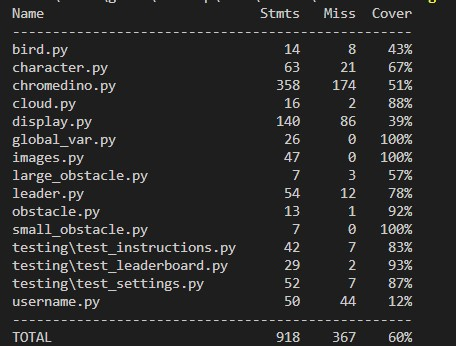
\includegraphics{coverage}
    \caption{Code coverage report}
    \label{fig:my_label}
\end{figure}




\bibliographystyle{plainnat}

\bibliography{SRS}

\end{document}